\adparagraph{Rating nDCG}
In Figure \ref{fig:andcg} we see the scores of the Rating nDCG measure. All methods generally have high levels of satisfaction according to the measure, with none scoring below 95 percent satisfaction.

Avg is ahead, but it is also the only method using the average rating of all the candidate items for its recommendation.

As can be seen in Table \ref{tbl:andcg}, BC, \MC, and SF do not decrease in score from 16 to 20, which is a curious result. SF even gains a little. In general, the fall in nDCG score is extremely low compared to the other measures. This is due to most, if not all of the candidate items being highly rated and this could indicates than even a random selection of movies could score highly on the Rating nDCG measure.

Among the remainder, while \MC does outperform both BC and SF, the difference is small.
\begin{figure}[H]
	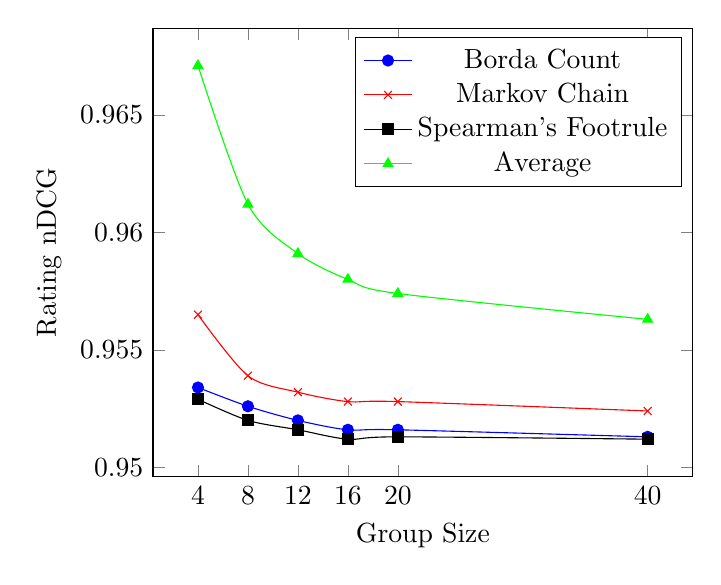
\begin{tikzpicture}
	\begin{axis}[
	y tick label style={
        /pgf/number format/.cd,
            precision=3,
        /tikz/.cd
    },
	xlabel=Group Size,
	ylabel=Rating nDCG,
	xtick = {4,8,12,16,20,40}]
	\addplot[smooth,mark=*,blue] plot coordinates {
		(4,0.9534)
		(8,0.9526)
		(12,0.952)
		(16,0.9516)
		(20,0.9516)
		(40,0.9513)
	};
	\addlegendentry{Borda Count}
	
	\addplot[smooth,color=red,mark=x] plot coordinates {
		(4,0.9565)
		(8,0.9539)
		(12,0.9532)
		(16,0.9528)
		(20,0.9528)
		(40,0.9524)
	};
	\addlegendentry{Markov Chain}
	
	\addplot[smooth,color=black,mark=square*] plot coordinates {
		(4,0.9529)
		(8,0.952)
		(12,0.9516)
		(16,0.9512)
		(20,0.9513)
		(40,0.9512)
	};
	\addlegendentry{Spearman's Footrule}
	
	\addplot[smooth,color=green,mark=triangle*] plot coordinates {
		(4,0.9671)
		(8,0.9612)
		(12,0.9591)
		(16,0.958)
		(20,0.9574)
		(40,0.9563)
	};
	\addlegendentry{Average}
	
	\end{axis}
	\end{tikzpicture}
	\caption{Results for Rating nDCG test}\label{fig:andcg}
\end{figure}

\begin{table}[H]
	\centering
	\begin{tabular}{|l|lllll|}\hline
		& 4 to 8 & 8 to 12 & 12 to 16 & 16 to 20 & 20 to 40 \\\hline
		BC 	& 0.084	& 0.063	& 0.42	& 0		& 0.032 \\
		MC  & 0.27	& 0.73	& 0.42	& 0		& 0.042 \\
		SF  & 0.094	& 0.042	& 0.042	&-0.011	& 0.011 \\
		Avg	& 0.61	& 0.22 	& 0.11	& 0.063	& 0.11  \\ \hline
	\end{tabular}
	\caption{Percentage decrease between the groups for Rating nDCG}
	\label{tbl:andcg}
\end{table}